%========================================================================
\section{Introduction}
%========================================================================
\IEEEPARstart{R}{etail} demand planning is one of the oldest and most economically important applications of data science. A large retailer such as Walmart must decide, every week and for every department of every store, how much stock to order, how many staff hours to schedule, and whether a promotion is worthwhile. The public \emph{Walmart Recruiting -- Store Sales Forecasting} dataset~\cite{kaggle_walmart} captures exactly this setting: 45 stores, 81 departments and almost three years of weekly sales, enriched with weather, fuel price, consumer price index (CPI), unemployment and five anonymised promotional ``MarkDown'' variables.

Most published studies on this dataset frame the task as point regression of weekly sales~\cite{chen2022,akande2022,yao2023,chenwi2024,punati2025}. Point forecasts, however, are notoriously noisy at the department level: sales are heavy-tailed, include negative values (returns), and the promotional variables are missing for most of the history. At the same time, many operational decisions are categorical in nature --- a store manager mainly needs to know whether next week will be a \emph{low}, \emph{medium} or \emph{high} volume week for a department in order to pick a staffing template or a replenishment tier. In this paper we therefore re-formulate the problem as a \textbf{three-class sales-level classification} task, with classes defined by the tertiles of the training distribution.

The reformulation also makes the dataset a demanding, realistic test-bed for the two families of techniques that dominate modern feature engineering: \emph{feature reduction} (projecting the data into a low-dimensional space) and \emph{feature selection} (choosing a subset of the original variables). The data are noisy, mixed-type (identifiers, binary flags, continuous macro-economic indicators) and only weakly structured in Euclidean space, so it is not obvious which techniques help. The contributions of this work are:

\begin{enumerate}
  \item A reproducible preprocessing pipeline and a noise audit of the dataset (Section~\ref{sec:data}), together with a three-class formulation of the sales-level problem.
  \item A side-by-side comparison of \textbf{ten} reduction methods --- three linear (PCA, LDA, SVD) and seven non-linear (Kernel PCA, SNE, t-SNE, UMAP, metric and non-metric MDS, Isomap, LLE) --- measured with three complementary criteria (neighbourhood classification accuracy, trustworthiness and class silhouette), plus a K-Means clustering analysis before and after reduction.
  \item A comparison of \textbf{four} feature-selection families: filter (variance, Spearman, ANOVA-F, $\chi^2$, mutual information with rank fusion), wrapper (sequential forward/backward selection and RFE), embedded (L1, L2, Elastic-Net logistic regression and gradient-boosting gain), and \textbf{metaheuristic} search with a Genetic Algorithm (GA), Binary Particle Swarm Optimisation (BPSO) and Simulated Annealing (SA) using a size-penalised fitness.
  \item A benchmark of nine classifiers under an 80/20 hold-out and stratified 5-fold cross-validation with the full set of metrics (confusion matrix, accuracy, error rate, precision, recall, F-measure, ROC-AUC), an explicit over-/under-fitting diagnosis, and a study of how every selected subset or projection affects the best model.
  \item Evidence that \emph{selection before reduction} --- running the embeddings only on the GA-selected variables --- markedly improves the class structure of the low-dimensional maps.
\end{enumerate}

The remainder of the paper is organised as follows. Section~\ref{sec:related} reviews related work. Section~\ref{sec:data} describes the data and preprocessing. Section~\ref{sec:methods} presents the methods. Section~\ref{sec:results} reports and interprets the results, Section~\ref{sec:compare} compares them with the literature, Section~\ref{sec:discussion} discusses limitations and Section~\ref{sec:conclusion} concludes.

%========================================================================
\section{Related Work}\label{sec:related}
%========================================================================
\subsection{Sales prediction on the Walmart dataset}
Chen~\cite{chen2022} compared multiple linear regression (MLR), Elastic-Net regression (ENR) and polynomial regression on the store-level version of the data and reported $R^2$ values of 0.933 (MLR) and 0.814 (ENR); the polynomial model reached a higher training $R^2$ but a test RMSE many orders of magnitude larger, a textbook case of over-fitting. Akande \emph{et al.}~\cite{akande2022} applied XGBoost to the 45-store data and concluded that gradient boosting is an effective forecaster. Yao~\cite{yao2023} compared decision-tree, random-forest and $k$-nearest-neighbour regressors on the department-level data; the random forest achieved $R^2=0.937$ and MAE $=1937.8$. Chenwi \emph{et al.}~\cite{chenwi2024} benchmarked linear regression, random forest, GBM, XGBoost and LightGBM and found XGBoost best (MAE $=1226.5$), also observing that errors are systematically larger for holiday weeks. More recently, Punati \emph{et al.}~\cite{punati2025} proposed a Temporal Fusion Transformer for multi-horizon probabilistic forecasting, reporting $R^2=0.9875$ and SMAPE $=4.51\%$ against XGBoost, CNN, LSTM and CNN-LSTM baselines.

Two observations motivate the present study. First, all of these works address regression; none studies a categorical sales-level formulation or reports classification metrics. Second, feature engineering in these works is largely manual: none systematically compares reduction methods or selection families, and none uses metaheuristic search over feature subsets.

\subsection{Feature reduction}
Linear reduction includes principal component analysis (PCA)~\cite{pearson1901}, which keeps the directions of maximum variance; linear discriminant analysis (LDA)~\cite{fisher1936}, which is supervised and maximises between-class relative to within-class scatter; and the singular value decomposition (SVD)~\cite{golub1970}, of which truncated SVD is the uncentred analogue of PCA. Non-linear methods either kernelise linear ones --- Kernel PCA~\cite{scholkopf1998} --- or preserve neighbourhood or distance structure. Stochastic Neighbor Embedding (SNE)~\cite{hinton2002} matches Gaussian neighbourhood probabilities in the input and output spaces; t-SNE~\cite{vandermaaten2008} symmetrises them and uses a heavy-tailed Student-$t$ kernel in the output space to alleviate the crowding problem; UMAP~\cite{mcinnes2018} builds a fuzzy topological graph and optimises a cross-entropy layout. Multidimensional scaling preserves pairwise distances either metrically~\cite{torgerson1952} or only through their rank order (non-metric MDS)~\cite{kruskal1964}; Isomap~\cite{tenenbaum2000} replaces Euclidean distances with graph geodesics, and Locally Linear Embedding (LLE)~\cite{roweis2000} preserves local linear reconstruction weights.

\subsection{Feature selection}
Following Guyon and Elisseeff~\cite{guyon2003}, selection methods are grouped into filters, wrappers and embedded methods. Filters score variables independently of any model, for instance by correlation, ANOVA-F, $\chi^2$ or mutual information~\cite{peng2005}. Wrappers~\cite{kohavi1997} search over subsets and score each with a learning algorithm; sequential forward/backward selection and recursive feature elimination (RFE)~\cite{guyon2002} are the classic greedy variants. Embedded methods select during training, e.g.\ through L1 (Lasso)~\cite{tibshirani1996}, L2 (Ridge)~\cite{hoerl1970} or Elastic-Net~\cite{zou2005} penalties, or through tree-ensemble importance. Because subset search is NP-hard, population-based metaheuristics are widely used: Genetic Algorithms~\cite{holland1975,goldberg1989,yang1998}, Binary PSO~\cite{kennedy1997} and Simulated Annealing~\cite{kirkpatrick1983}; Xue \emph{et al.}~\cite{xue2016} survey evolutionary approaches and note that their main weakness is computational cost, which we mitigate here through subsampling, a fast surrogate learner and fitness caching.

%========================================================================
\section{Dataset and Preprocessing}\label{sec:data}
%========================================================================
\subsection{Source data}
The data come from the Kaggle competition \emph{Walmart Recruiting -- Store Sales Forecasting}~\cite{kaggle_walmart} and consist of three related tables. The \texttt{train} table holds 421{,}570 department-week records (\texttt{Store}, \texttt{Dept}, \texttt{Date}, \texttt{Weekly\_Sales}, \texttt{IsHoliday}) for 45 stores and 81 departments, from 5~February~2010 to 26~October~2012. The \texttt{features} table adds, for every store-week, the average regional \texttt{Temperature}, the regional \texttt{Fuel\_Price}, five anonymised promotional variables \texttt{MarkDown1}--\texttt{MarkDown5}, the \texttt{CPI} and the regional \texttt{Unemployment} rate. The \texttt{stores} table gives each store's \texttt{Type} (A, B or C) and floor \texttt{Size}. The three tables are joined on (\texttt{Store}, \texttt{Date}) and \texttt{Store}, respectively. The four holiday weeks flagged by Walmart --- Super Bowl, Labor Day, Thanksgiving and Christmas --- are known to be weighted five times more heavily in the original competition metric.

\subsection{Noise audit}
The cover specification of this project asks for a ``difficult dataset with noise''. Table~\ref{tab:noise} quantifies why the Walmart data qualify. The target is extremely right-skewed (skewness 3.26; mean \$15{,}981 versus median \$7{,}612; maximum \$693{,}099). 1{,}285 records have \emph{negative} sales (net returns), and 35{,}521 records (8.4\%) lie outside the $1.5\times$IQR whiskers. The promotional variables are missing for 64--74\% of the rows, mostly because MarkDowns were only recorded from November 2011 onward, and 1{,}568 MarkDown values are negative, which is impossible for a discount amount and must be treated as entry errors. Finally, the store-week context variables (temperature, fuel price, CPI, unemployment) are measured at the store or region level and are therefore identical for all $\approx$74 departments of a store in a given week: for the department-level target they act as weak, highly redundant covariates.

\begin{table}[!t]
\caption{Noise and quality issues in the merged dataset (421{,}570 rows)}
\label{tab:noise}
\centering
\begin{tabular}{lrr}
\toprule
Issue & Count & \% rows \\
\midrule
Negative weekly sales (returns) & 1{,}285 & 0.30 \\
Weekly-sales outliers ($1.5\times$IQR) & 35{,}521 & 8.43 \\
MarkDown1 missing & 270{,}889 & 64.26 \\
MarkDown2 missing & 310{,}322 & 73.61 \\
MarkDown3 missing & 284{,}479 & 67.48 \\
MarkDown4 missing & 286{,}603 & 67.98 \\
MarkDown5 missing & 270{,}138 & 64.08 \\
Negative MarkDown values & 1{,}568 & 0.37 \\
Holiday-week rows & 29{,}661 & 7.04 \\
Skewness of \texttt{Weekly\_Sales} & \multicolumn{2}{c}{3.26} \\
\bottomrule
\end{tabular}
\end{table}

\subsection{Target definition}
We define three ordered classes by the 33.3th and 66.7th percentiles of \texttt{Weekly\_Sales}: \textbf{Low} ($\le\$3{,}521.78$), \textbf{Medium} ($\$3{,}521.78$--$\$14{,}599.76$) and \textbf{High} ($>\$14{,}599.76$). By construction the classes are balanced (140{,}524 / 140{,}523 / 140{,}523 rows), so accuracy is a meaningful headline metric and the chance level is 33.3\%. Negative sales are kept --- they are genuine business events --- and fall into the Low class.

\subsection{Preprocessing}
\begin{enumerate}
\item \textbf{Missing promotions.} A missing MarkDown means that no promotion was recorded, so it is replaced by zero, and a binary \texttt{MarkDown\_Available} flag preserves the information that the value was missing.
\item \textbf{Promotion noise.} Negative MarkDowns are clipped to zero, and each MarkDown is winsorised at its 99.5th percentile to limit the leverage of extreme promotions.
\item \textbf{Calendar features.} From \texttt{Date} we derive \texttt{Year}, \texttt{Month}, ISO \texttt{Week} and \texttt{Day}; the signed number of days to Thanksgiving and to Christmas of the same year; and binary Super Bowl and Labor Day indicators.
\item \textbf{Encoding.} Store \texttt{Type} is one-hot encoded (\texttt{Type\_A}, \texttt{Type\_B}, \texttt{Type\_C}) and \texttt{IsHoliday} is cast to an integer.
\end{enumerate}
The final design matrix has \textbf{25 features}, listed in Table~\ref{tab:features}, and no missing values.

\begin{table}[!t]
\caption{The 25 model features}
\label{tab:features}
\centering
\begin{tabular}{p{1.9cm}p{5.9cm}}
\toprule
Group & Features \\
\midrule
Identity & Store, Dept \\
Store & Size, Type\_A, Type\_B, Type\_C \\
Economy & Temperature, Fuel\_Price, CPI, Unemployment \\
Promotion & MarkDown1--5, MarkDown\_Available \\
Calendar & IsHoliday, Year, Month, Week, Day, Days\_to\_Thanksgiving, Days\_to\_Christmas, SuperBowl, LaborDay \\
\bottomrule
\end{tabular}
\end{table}

\subsection{Exploratory analysis}
Fig.~\ref{fig:eda} summarises the data before any reduction. Total chain-wide sales are flat for most of the year and spike sharply in the flagged Thanksgiving week (about \$66M versus a typical \$45--50M) and in the week \emph{before} Christmas (up to \$81M). The flagged Christmas week itself, which ends on the last Friday of December, is actually a dip, and the Super Bowl and Labor Day weeks show no visible spike. Only one of the four official holiday weeks therefore coincides with a peak, which already hints that the \texttt{IsHoliday} flag is a weak predictor. Store size increases from Type C to Type A stores; within Types A and B the High class is associated with larger stores, whereas Type C stores all have almost the same size. Fig.~\ref{fig:corr} shows the Spearman correlation matrix: the strongest monotone association with the sales class is \texttt{Size} ($\rho=0.26$), followed by the store-type dummies ($|\rho|=0.10$--$0.19$); all other features have $|\rho|<0.08$. In particular, \texttt{Dept} has an almost zero rank correlation with the class ($\rho=-0.03$) even though, as shown later, it is by far the most informative variable: its effect is strong but entirely \emph{non-monotone}, because department numbers are arbitrary identifiers. The calendar variables \texttt{Week}, \texttt{Month}, \texttt{Days\_to\_Thanksgiving} and \texttt{Days\_to\_Christmas} are almost perfectly collinear, and so are the five MarkDowns, which indicates substantial redundancy for the reduction and selection methods to exploit.

\begin{figure*}[!t]
\centering
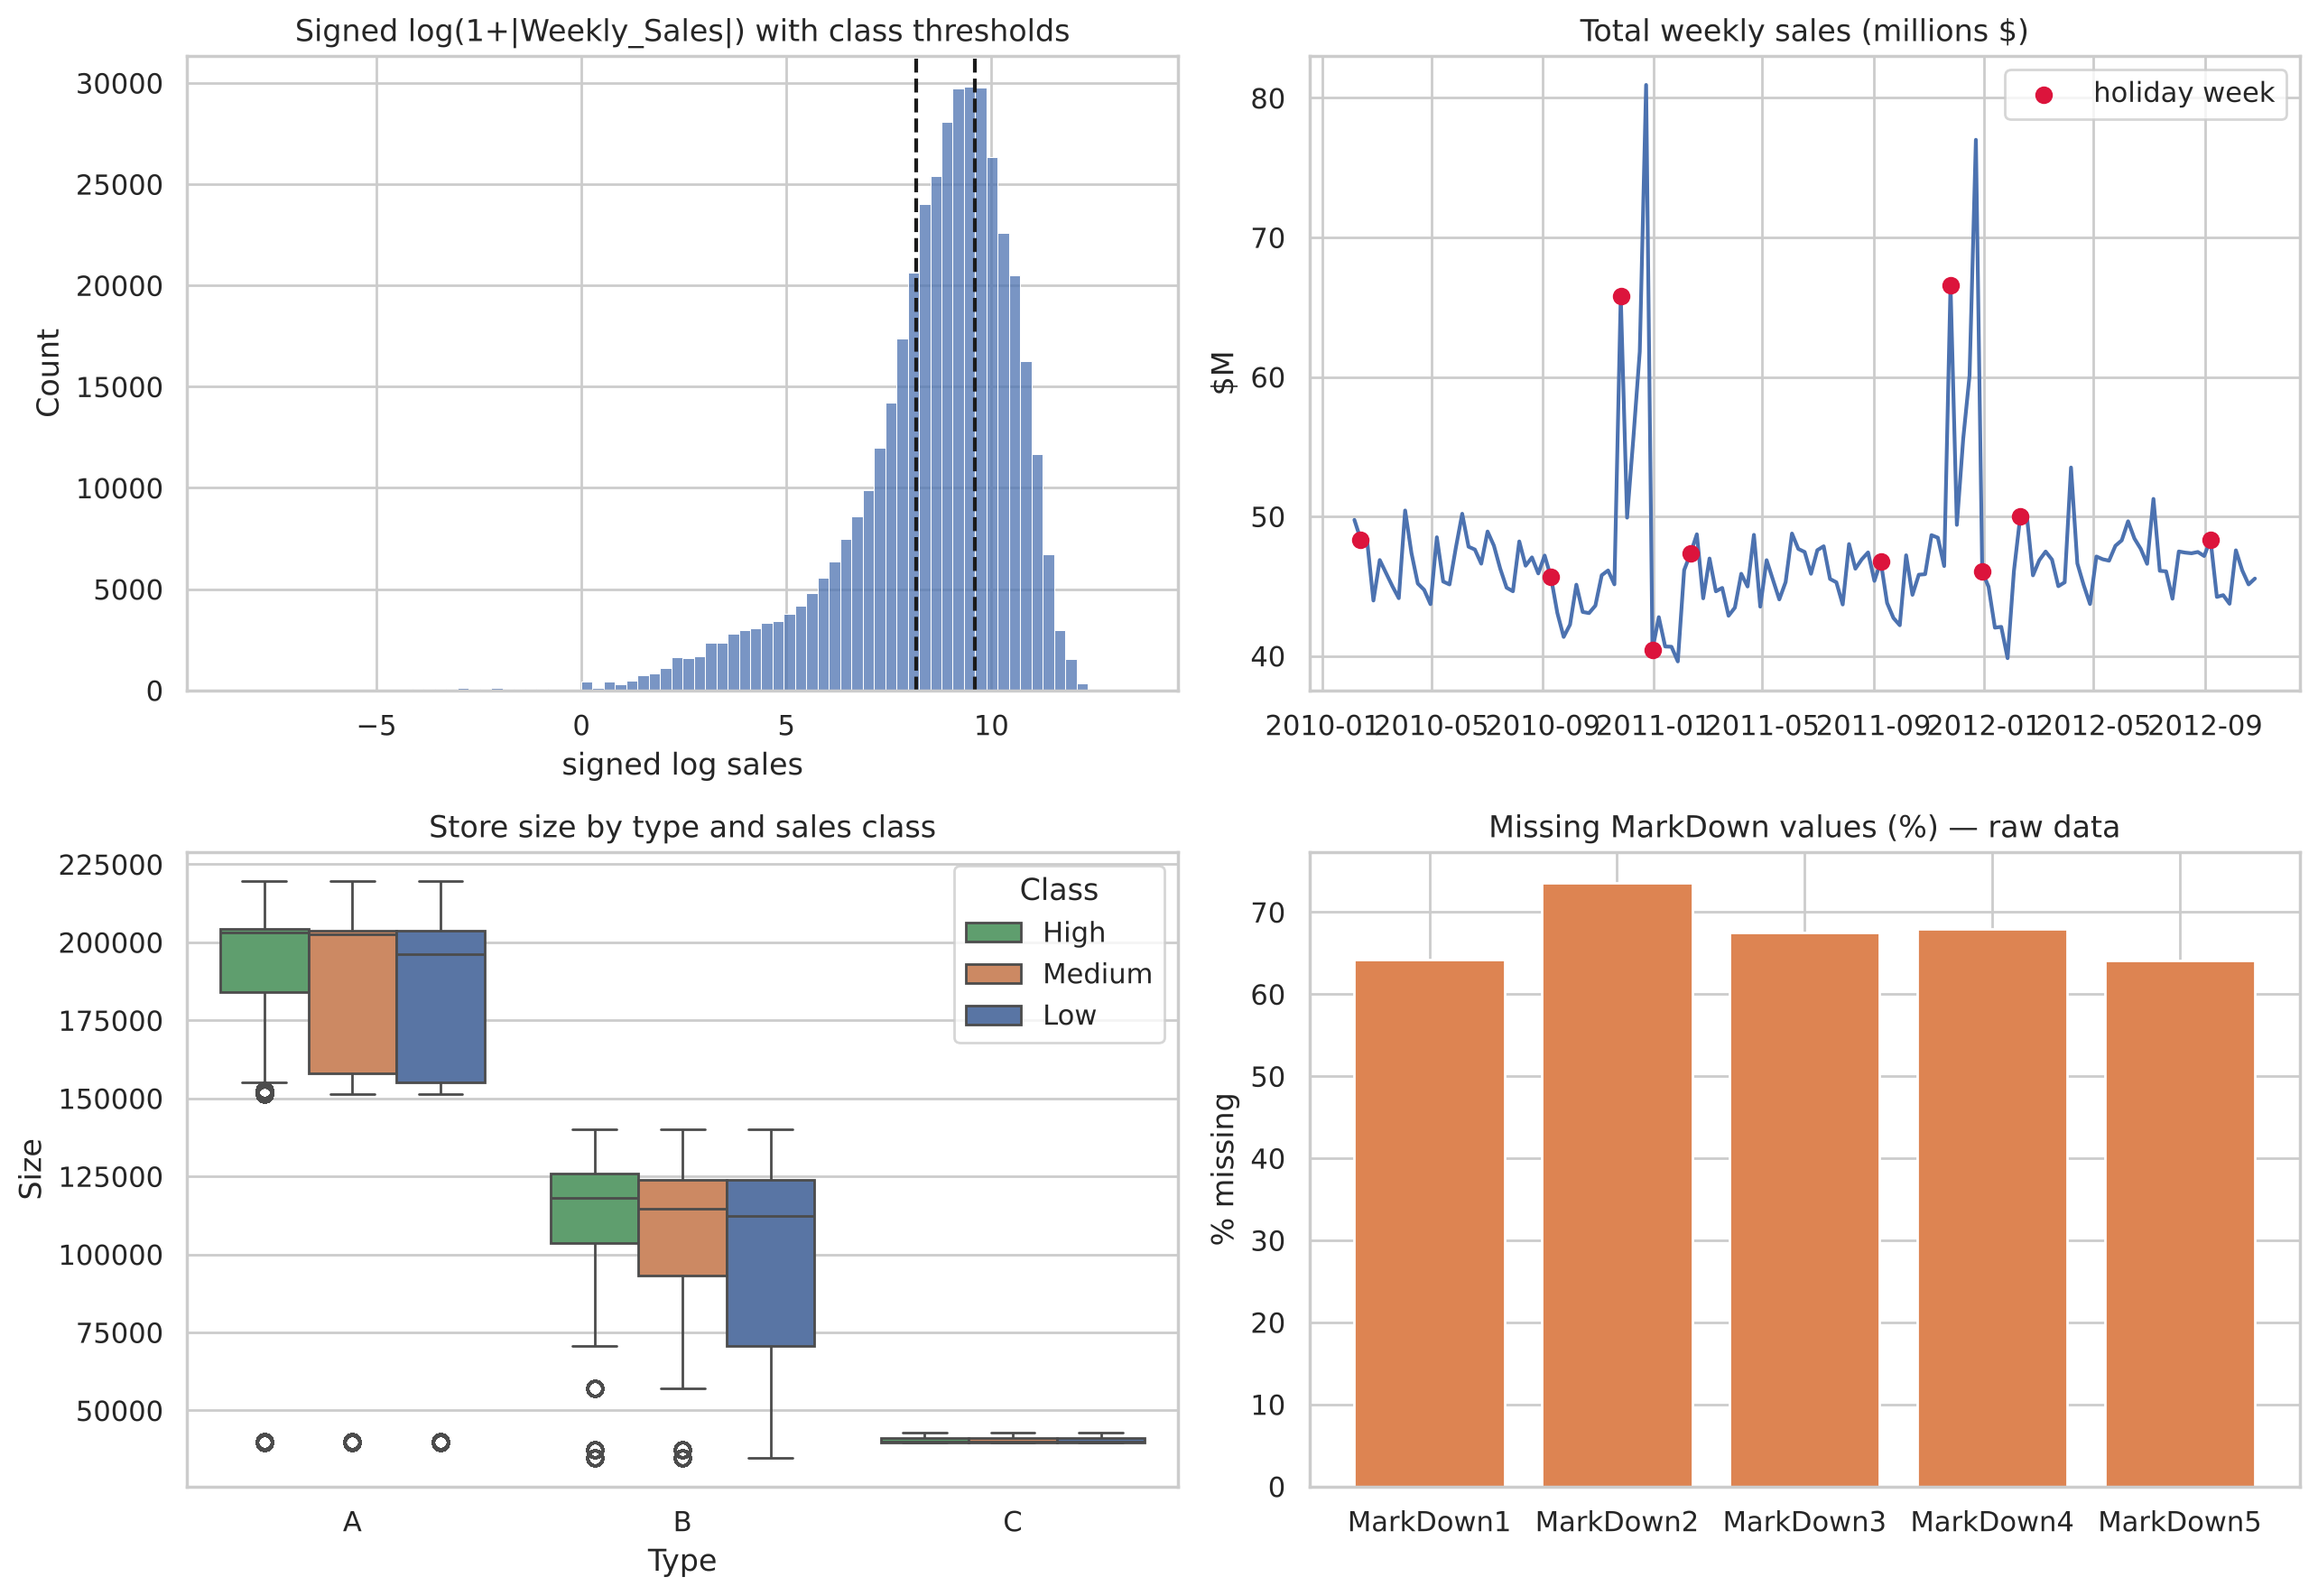
\includegraphics[width=0.86\textwidth]{figures/01_eda_overview.png}
\caption{Exploratory analysis before reduction. Top-left: signed $\log(1+|\text{sales}|)$ with the two class thresholds (dashed). Top-right: chain-wide weekly sales with holiday weeks in red. Bottom-left: store size by type and class. Bottom-right: share of missing MarkDown values in the raw data.}
\label{fig:eda}
\end{figure*}

\begin{figure}[!t]
\centering
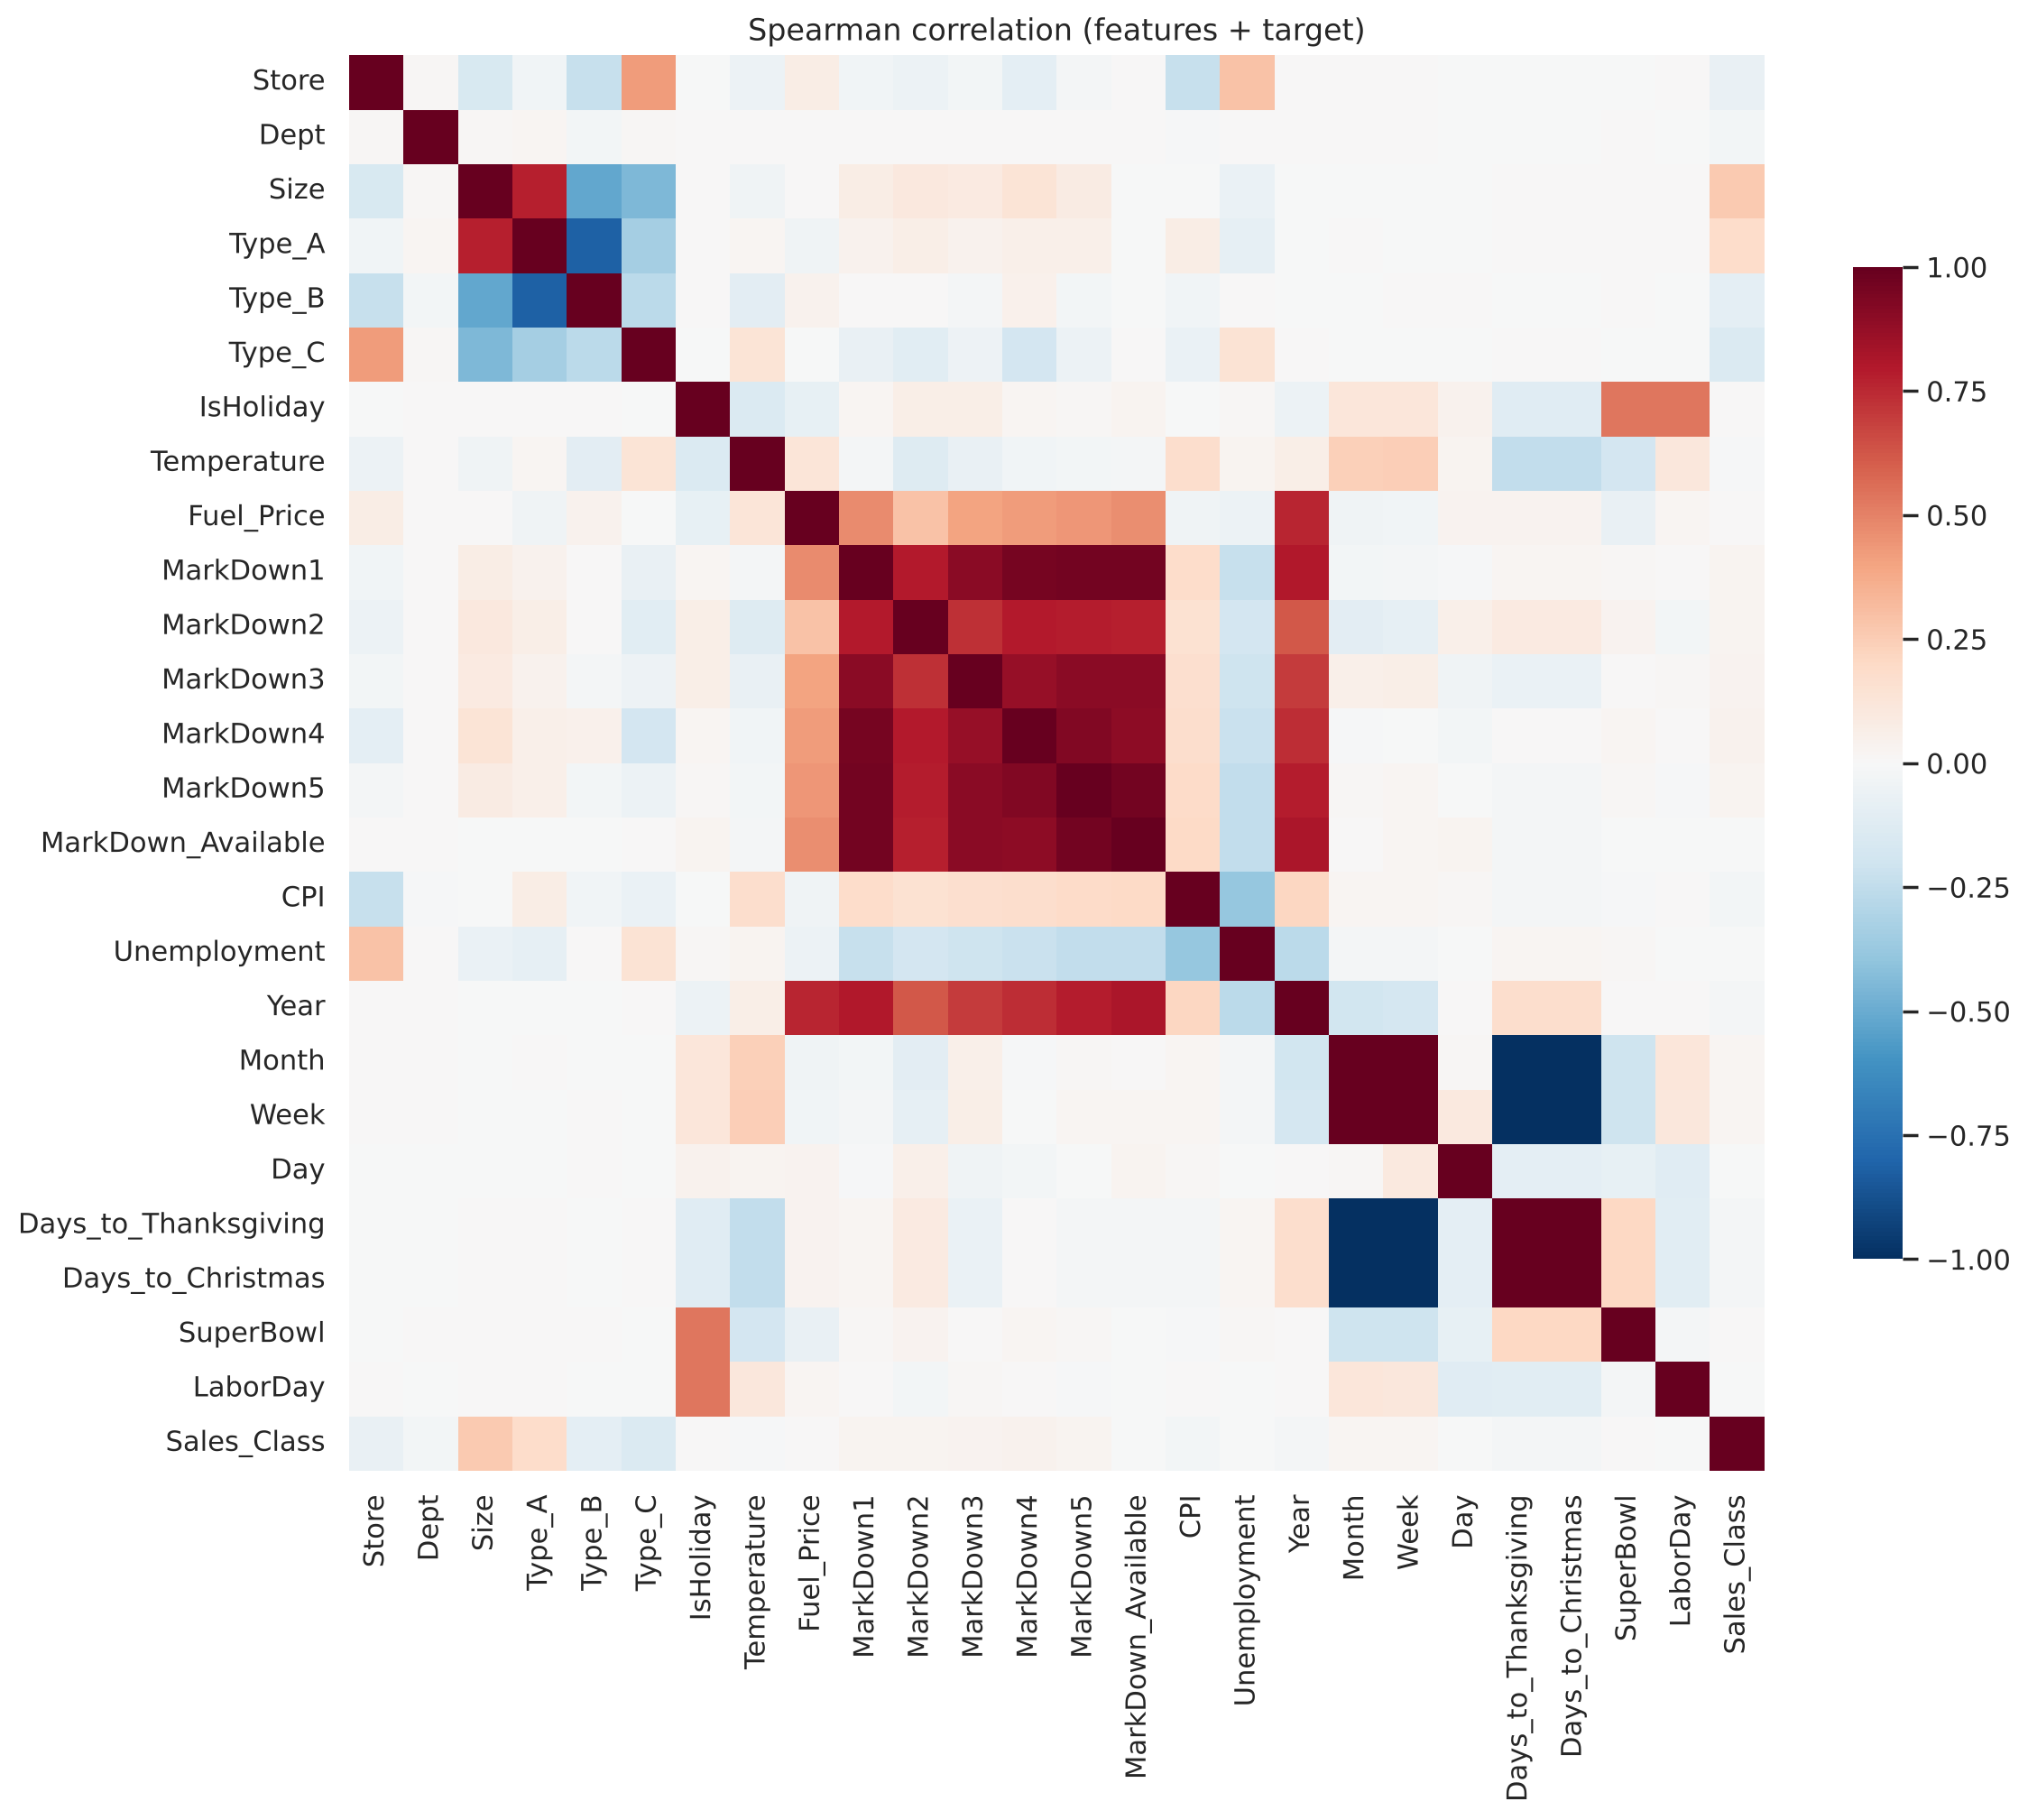
\includegraphics[width=\columnwidth]{figures/02_correlation.png}
\caption{Spearman correlation between the 25 features and the ordinal sales class (last row/column).}
\label{fig:corr}
\end{figure}

\subsection{Sampling and splitting}
Training nine models with 5-fold cross-validation, and running three metaheuristics that each evaluate several hundred feature subsets, on 421{,}570 rows is beyond the two-core, 8-GB machine used for this study. We therefore draw a \textbf{stratified sample of 100{,}000 rows} (23.7\% of the data) and split it \textbf{80/20} with stratification into 80{,}000 training and 20{,}000 test rows. Feature selection uses a 20{,}000-row subsample of the training split only, so the test rows never influence which features are chosen. The manifold methods, whose cost grows quadratically or cubically with $n$, use a 3{,}000-point subsample of the training split (1{,}500 points for SNE and 1{,}000 for MDS).


%========================================================================
\section{Methodology}\label{sec:methods}
%========================================================================
Fig.~\ref{fig:pipeline} summarises the experimental pipeline. All randomness is controlled with a single seed (42) and all experiments were run with scikit-learn~\cite{pedregosa2011}, LightGBM~\cite{ke2017}, XGBoost~\cite{chen2016xgb} and umap-learn~\cite{mcinnes2018}. The complete code is available in the accompanying Jupyter notebook.

\begin{figure}[!t]
\centering
\begin{tikzpicture}[node distance=0.32cm, every node/.style={font=\scriptsize},
  box/.style={draw, rounded corners, fill=blue!6, text width=7.9cm, minimum height=0.55cm, align=center},
  arr/.style={-{Stealth[length=2mm]}, thick}]
\node[box] (a) {Raw data: train + features + stores (421{,}570 dept-weeks)};
\node[box, below=of a] (b) {Noise audit $\rightarrow$ preprocessing $\rightarrow$ 25 features; 3-class target (tertiles)};
\node[box, below=of b] (c) {Stratified 100k sample $\rightarrow$ 80\% train / 20\% test};
\node[box, below=of c, fill=green!6] (d) {Reduction (3{,}000-pt sample): PCA, LDA, SVD, KPCA, SNE, t-SNE, UMAP, MDS$\times$2, Isomap, LLE + K-Means};
\node[box, below=of d, fill=orange!8] (e) {Selection (20k train rows): filter $|$ wrapper $|$ embedded $|$ GA, BPSO, SA};
\node[box, below=of e, fill=red!6] (f) {9 classifiers $\rightarrow$ hold-out, 5-fold CV, CM, ROC, learning curves};
\node[box, below=of f] (g) {Best model re-trained on every subset / projection; comparison with literature};
\foreach \u/\v in {a/b,b/c,c/d,d/e,e/f,f/g} \draw[arr] (\u) -- (\v);
\end{tikzpicture}
\caption{Experimental pipeline. Feature selection only ever sees training rows; the 20\% test split is touched once per model.}
\label{fig:pipeline}
\end{figure}

\subsection{Linear reduction}
Let $\mathbf{X}\in\mathbb{R}^{n\times d}$ be the standardised data matrix. \textbf{PCA} computes the eigen-decomposition of the covariance $\mathbf{C}=\frac{1}{n-1}\mathbf{X}^\top\mathbf{X}=\mathbf{V}\boldsymbol{\Lambda}\mathbf{V}^\top$ and projects onto the $k$ leading eigenvectors, $\mathbf{Z}=\mathbf{X}\mathbf{V}_k$; the explained-variance ratio of component $j$ is $\lambda_j/\sum_i\lambda_i$. \textbf{LDA} solves the generalised eigenproblem $\mathbf{S}_B\mathbf{w}=\lambda\mathbf{S}_W\mathbf{w}$ with between-class scatter $\mathbf{S}_B=\sum_c n_c(\boldsymbol{\mu}_c-\boldsymbol{\mu})(\boldsymbol{\mu}_c-\boldsymbol{\mu})^\top$ and within-class scatter $\mathbf{S}_W=\sum_c\sum_{i\in c}(\mathbf{x}_i-\boldsymbol{\mu}_c)(\mathbf{x}_i-\boldsymbol{\mu}_c)^\top$; with $C=3$ classes it yields at most $C-1=2$ discriminant axes. \textbf{Truncated SVD} factorises $\mathbf{X}\approx\mathbf{U}_k\boldsymbol{\Sigma}_k\mathbf{V}_k^\top$ and keeps $\mathbf{Z}=\mathbf{U}_k\boldsymbol{\Sigma}_k$; on centred data it coincides with PCA, which serves as a sanity check.

\subsection{Non-linear reduction}
\textbf{Kernel PCA} performs PCA in a feature space induced by the RBF kernel $k(\mathbf{x},\mathbf{x}')=\exp(-\gamma\|\mathbf{x}-\mathbf{x}'\|^2)$ by eigen-decomposing the centred Gram matrix; $\gamma$ was chosen from $\{0.005,0.02,0.05,0.1\}$ by kNN accuracy. \textbf{SNE} defines conditional probabilities
\begin{equation}
p_{j|i}=\frac{\exp(-\|\mathbf{x}_i-\mathbf{x}_j\|^2/2\sigma_i^2)}{\sum_{k\neq i}\exp(-\|\mathbf{x}_i-\mathbf{x}_k\|^2/2\sigma_i^2)},
\end{equation}
with $\sigma_i$ found by binary search so that the perplexity $2^{H(P_i)}$ equals 30, analogous Gaussian $q_{j|i}$ in the 2-D space, and minimises $\sum_i \mathrm{KL}(P_i\|Q_i)$ whose gradient is
\begin{equation}
\frac{\partial C}{\partial\mathbf{y}_i}=2\sum_j\left(p_{j|i}-q_{j|i}+p_{i|j}-q_{i|j}\right)(\mathbf{y}_i-\mathbf{y}_j).
\end{equation}
Because scikit-learn does not provide SNE, we implemented it from scratch (gradient descent with momentum 0.5$\to$0.8, learning rate 0.1, 600 iterations, gradient clipping to protect against ``hub'' points). \textbf{t-SNE} uses symmetric joint probabilities and the Student-$t$ output kernel $q_{ij}\propto(1+\|\mathbf{y}_i-\mathbf{y}_j\|^2)^{-1}$ (perplexity 30, PCA initialisation). \textbf{UMAP} uses 15 neighbours and a minimum distance of 0.1. \textbf{Metric MDS} minimises the raw stress $\sum_{i<j}(\|\mathbf{y}_i-\mathbf{y}_j\|-\delta_{ij})^2$ with the SMACOF algorithm; \textbf{non-metric MDS} replaces $\delta_{ij}$ by a monotone (isotonic) transformation of it. \textbf{Isomap} (10 neighbours) applies classical MDS to shortest-path distances on the $k$NN graph, and \textbf{LLE} (12 neighbours) finds weights $\mathbf{W}$ minimising $\sum_i\|\mathbf{x}_i-\sum_j W_{ij}\mathbf{x}_j\|^2$ and then low-dimensional points preserving the same weights.

\subsection{Embedding quality criteria}
Because a 2-D picture can be misleading, every embedding is scored with three numbers: (i) the 5-fold accuracy of a 5-NN classifier trained \emph{in} the embedding, which measures how much class information survives; (ii) trustworthiness~\cite{venna2006},
\begin{equation}
T(k)=1-\frac{2}{nk(2n-3k-1)}\sum_{i=1}^{n}\sum_{j\in U_i^{(k)}}\left(r(i,j)-k\right),
\end{equation}
where $U_i^{(k)}$ are points that are among the $k=10$ nearest neighbours of $i$ in the embedding but not in the input space and $r(i,j)$ is their rank in the input space; and (iii) the silhouette~\cite{rousseeuw1987} of the true classes. For clustering we run K-Means~\cite{lloyd1982} with $k=3$ and report the silhouette of the found clusters together with the Adjusted Rand Index (ARI)~\cite{hubert1985} and normalised mutual information (NMI) against the true sales classes.

\subsection{Feature selection}
All selectors operate on a 20{,}000-row subsample of the \emph{training} split; subset sizes for ranked or greedy methods are fixed at $K=10$ of 25 features.

\textbf{Filter.} For every feature we compute the variance after min--max scaling, the absolute Spearman correlation with the ordinal class, the ANOVA $F$ statistic, the $\chi^2$ statistic on min--max scaled values and the mutual information (with discrete treatment for variables having fewer than 60 distinct values). The four relevance scores are converted to ranks and averaged (\emph{rank fusion}); the ten best-ranked features form the filter subset.

\textbf{Wrapper.} Sequential forward selection (SFS) starts from the empty set and greedily adds the feature that most improves the 3-fold macro-F1 of a fast LightGBM (60 trees); sequential backward selection starts from all features and removes greedily. RFE repeatedly fits a 60-tree random forest and drops the least important feature.

\textbf{Embedded.} Multinomial logistic regression with $C=0.05$ is trained on standardised data under three penalties,
\begin{equation}
\Omega(\mathbf{W})=\alpha\|\mathbf{W}\|_1+\tfrac{1-\alpha}{2}\|\mathbf{W}\|_2^2,\quad \alpha\in\{1,\,0,\,0.5\},
\end{equation}
i.e.\ L1 (Lasso), L2 (Ridge) and Elastic-Net. A feature is kept by L1/Elastic-Net if the norm of its coefficient vector across the three classes is non-zero; for L2, which never produces exact zeros, the ten largest norms are kept. LightGBM total-gain importance is reported as a tree-based embedded reference.

\textbf{Metaheuristics.} A candidate solution is a bit-mask $\mathbf{b}\in\{0,1\}^{25}$. All three searches maximise the same fitness
\begin{equation}
f(\mathbf{b})=\overline{F_1}^{\,3\text{-fold}}(\mathbf{b})-\lambda\frac{\|\mathbf{b}\|_1}{25},\qquad \lambda=0.02,
\label{eq:fitness}
\end{equation}
which trades predictive quality against subset size; evaluated masks are cached so that repeated individuals cost nothing. The \textbf{GA} uses a population of 24, 20 generations, tournament selection ($k=3$), uniform crossover ($p_c=0.9$), bit-flip mutation ($p_m=1/25$) and elitism of two. \textbf{BPSO} uses 20 particles and 20 iterations with inertia $w=0.7$, $c_1=c_2=1.5$, velocity clamp $\pm4$ and the sigmoid transfer $P(b_{id}=1)=1/(1+e^{-v_{id}})$. \textbf{SA} performs 300 single-bit-flip moves with initial temperature $T_0=0.02$, geometric cooling $\alpha=0.985$ and the Metropolis acceptance rule $P=\exp(\Delta f/T)$.

\subsection{Classifiers}
Nine classifiers cover linear, probabilistic, instance-based, single-tree, bagging, boosting and neural families: logistic regression; Gaussian naive Bayes; $k$-NN ($k=15$); an unpruned decision tree; random forest~\cite{breiman2001} (150 trees, minimum leaf size 2); extra trees~\cite{geurts2006} (150 trees, minimum leaf size 2); a multilayer perceptron (128--64 ReLU units, early stopping); XGBoost~\cite{chen2016xgb} (400 trees, depth 8, learning rate 0.1, row/column subsampling 0.9); and LightGBM~\cite{ke2017} (500 trees, 127 leaves, learning rate 0.05). Scale-sensitive models are wrapped in a standardisation pipeline fitted on the training fold only.

\subsection{Evaluation protocol}
From the 421{,}570 rows we draw a stratified sample of 100{,}000 and split it 80/20 with stratification. On the 20\% test set we report the confusion matrix and
\begin{align}
\text{Accuracy}&=\tfrac{\sum_c TP_c}{N},\qquad \text{Error rate}=1-\text{Accuracy},\\
\text{Precision}&=\tfrac{1}{C}\sum_c\tfrac{TP_c}{TP_c+FP_c},\quad \text{Recall}=\tfrac{1}{C}\sum_c\tfrac{TP_c}{TP_c+FN_c},\\
F_1&=\tfrac{1}{C}\sum_c\tfrac{2P_cR_c}{P_c+R_c},
\end{align}
(macro averages) and the one-vs-rest macro ROC-AUC~\cite{fawcett2006}. Stratified 5-fold cross-validation~\cite{kohavi1995} on the full 100k sample gives the mean and standard deviation of accuracy, macro-F1 and AUC. A model is labelled \emph{over-fitting} when its train--test accuracy gap exceeds 5 percentage points, and \emph{under-fitting} when its test accuracy is below 70\% with a small gap. Learning curves of the best model and a validation curve of the decision-tree depth make the bias--variance behaviour visible.
